\documentclass[12pt,a4paper]{article}
\usepackage[utf8x]{inputenc}
\usepackage{ucs}
\usepackage{amsmath}
\usepackage{amsfonts}
\usepackage{amssymb}
\usepackage{graphicx}
\usepackage{grffile}
\usepackage{float}
\usepackage{multicol}
\usepackage[portuguese]{babel}
\title{MAT2456 P1-2015}
\author{André Garnier Coutinho}
\setlength{\textwidth}{17cm}
\setlength{\textheight}{24cm}
\addtolength{\topmargin}{-2cm}
\addtolength{\oddsidemargin}{-2cm}

\newcommand{\re}{\mathbb{R}}

\newcommand{\sen}{\mbox{\, sen}\,}

\begin{document}
%%%%%%%%%%%%%%%%%%%%%%%%%%%%%%%%%%%%%%%%%%TURMA A%%%%%%%%%%%%%%%%%%%%%%%%%%%%%%%%%%%%%%%%%%%%%%%
\begin{center}
\textbf{Instituto de Matemática e Estatística da USP\\
MAT2455 - Cálculo Diferencial e Integral IV para Engenharia\\}
\textbf{1a. Prova - 2o. Semestre 2015 - 07/04/2015}
\end{center}

\noindent {\bf Turma A}

%---------------------------------------QUESTAO 1-----------------------------------------

\noindent{\bf 1ª Questão:}
\begin{itemize}
	\item[a)] (1,5) Calcule a área de um laço da rosácea cuja equação em coordenadas polares é $r(\theta) = \cos 5\theta$. \\
	\item[b)] (2,0) Calcule  $\displaystyle\iint_D \frac{x+y-1}{x+y+1}\; \, dx \, dy$, sendo $D$ a região do plano limitada por:
	$$ x+y-1 = x-y+1, \; x+y-1= 2(x-y+1), \; x-y+1=1, \; x-y+1 = 2.$$
	
\end{itemize}


\noindent{\bf \\ \\Solução:}
\begin{itemize}
    \item[a)] O laço da rosácea em questão apresenta o seguinte formato:
    

\begin{figure}[h!]
	\centering
	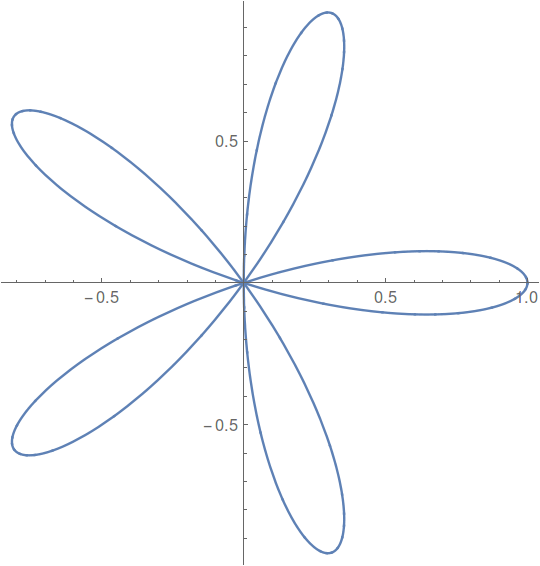
\includegraphics[scale=0.40]{Fig1.png}  
	\caption{Laço da rosácea}
	\label{fig:figura1}
\end{figure}

Como cada laço começa e termina em $r=0$ e $r \geq 0 \Rightarrow \cos 5\theta \geq 0$, deve existir um laço em $-\frac{\pi}{2} \leq 5\theta \leq \frac{\pi}{2} \Rightarrow -\frac{\pi}{10} \leq \theta \leq \frac{\pi}{10}$. Logo, a área de um laço da rosácea é dada por:

$$ \int\limits_{-\frac{\pi}{10}}^{\frac{\pi}{10}} \int\limits_0^{\cos 5\theta} \rho \; d\rho \, d\theta = \int\limits_{-\frac{\pi}{10}}^{\frac{\pi}{10}} \frac{\rho^2}{2} \Big|_0^{\cos 5\theta} \; d\theta = \frac{1}{2} \int\limits_{-\frac{\pi}{10}}^{\frac{\pi}{10}} \cos^2(5\theta) \; d\theta = \frac{1}{2} \int\limits_{-\frac{\pi}{10}}^{\frac{\pi}{10}} \frac{1 + \cos (10\theta)}{2} \; d\theta $$
$$ = \frac{1}{4} \Big( \theta + \frac{\sin (10\theta)}{10} \Big)_{-\frac{\pi}{10}}^{\frac{\pi}{10}} = \frac{1}{4} \cdot \frac{\pi}{5} = \frac{\pi}{20} $$

\item[b)] O domínio de integração é exibido abaixo

\begin{figure}[H]
	\centering
	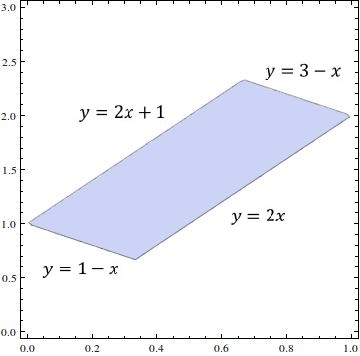
\includegraphics[scale=0.4]{Q1bA.jpg}  
	\caption{Domínio de integração}
	\label{fig:figura2}
\end{figure}    
Faz-se a seguinte mudança de coordenadas:
$$\begin{cases}
u = x+y-1\\
v = x-y+1
\end{cases}
\Rightarrow
\begin{cases}
x = \frac{u+v}{2}\\
y = \frac{u-v}{2}+1
\end{cases}
$$

O jacobiano da transformação é dado por:
$$
\frac{\partial(x,y)}{\partial(u,v)}=
\begin{vmatrix}
\frac{1}{2} & \frac{1}{2} \\
\frac{1}{2} & -\frac{1}{2}\\
\end{vmatrix}
=-\frac{1}{2} \Rightarrow |J|=\frac{1}{2}\\
$$  

O novo domínio de integração é exibido abaixo

\begin{figure}[h!]
	\centering
	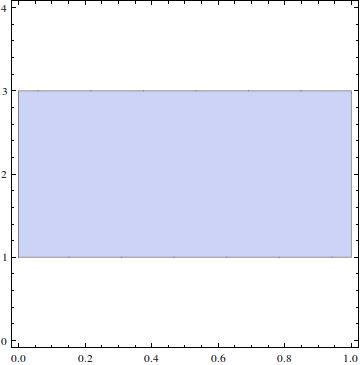
\includegraphics[scale=0.4]{Q1b2A.jpg}  
	\caption{Domínio de integração após mudança}
	\label{fig:figura3}
\end{figure}
E passa a ser dado por:

$$D(u,v)=\{(u,v)\in \re^2|v \leq u \leq 2v\,\,\mbox{,}\,\,1 \leq v \leq 2 \}$$

A integral a ser calculada passa a ser:

$$ \int\limits_1^2 \int\limits_v^{2v} \frac{u}{v^4} \cdot \frac{1}{2} \; du \, dv = \frac{1}{2} \int\limits_1^2  \frac{u^2}{2} \Big|_v^{2v} \frac{1}{v^4}  \; dv = \frac{1}{4} \int\limits_1^2  \frac{4v^2 - v^2}{v^4}  \; dv = \frac{3}{4} \int\limits_1^2  \frac{1}{v^2}  \; dv = \frac{3}{4} \cdot \frac{v^{-1}}{-1} \Big|_1^2 = -\frac{3}{4} \Big( \frac{1}{2} -1 \Big) = \frac{3}{8} $$

\end{itemize}

%---------------------------------------QUESTAO 2-----------------------------------------
\newpage

\noindent{\bf 2ª Questão:}

\begin{itemize}
\item[a)] (2,0) Calcule a massa da curva cujo traço é a parte da elipse $\displaystyle\frac{x^2}{3} + \displaystyle\frac{y^2}{4} = 1 $ no primeiro quadrante com densidade $\delta(x,y) = xy$. \\
\item[b)] (1,5) Inverta a ordem de integração e calcule a integral iterada: $\displaystyle\int_0^2 \int_{y^2}^4 y \frac{\ln (1+x^2)}{1+x^2} \; dx \, dy$.
\end{itemize}

\noindent{\bf Solução:} \\

\begin{itemize}
\item[a)]
Devemos calcular a integral
$$  \int_{\gamma}{\delta(x,y,z)}\;ds $$

\begin{figure}[h!]
	\centering
	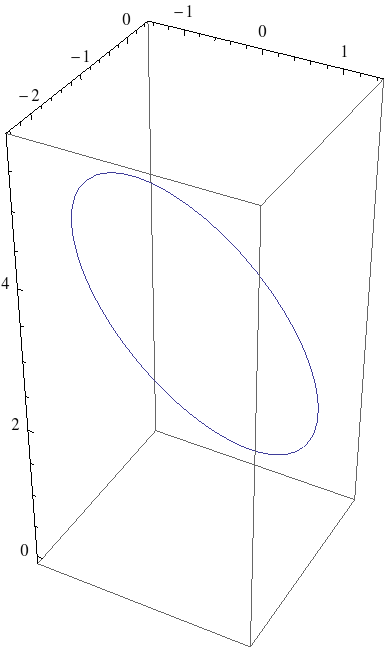
\includegraphics[scale=0.2]{Fig3.png}  
	\caption{Curva $\gamma(t)$}
	\label{fig:figura3}
\end{figure}

Parametrizando a curva em questão:

$$
\frac{x^2}{3} + \frac{y^2}{4} = 1
\Rightarrow
\begin{cases}
x(t) = \sqrt{3}\cos t \\
y(t) = 2\sin t\\
\end{cases}
$$

$$ \therefore \gamma(t) = (\sqrt{3}\cos t, 2\sin t), t \in \Big[0,\frac{\pi}{2}\Big] $$
$$ \gamma'(t) = (-\sqrt{3}\sin t, 2\cos t) $$
$$ ||\gamma'(t)|| = \sqrt{3\sin^2 t + 4\cos^2 t} = \sqrt{1 + \cos^2 t} $$

Utilizando a definição de integral de linha de uma função escalar:

$$  \int_{\gamma}{\delta(x,y)}\;ds = \int_{t_i}^{t_f} {\delta(\gamma(t)) ||\gamma'(t) ||}\;dt = \int_{0}^{\frac{\pi}{2}} 2 \sqrt{3} \, \sin t \cos t \sqrt{1 + \cos^2 t} \;dt $$

Utilizando a seguinte mudança de váriavel: $u = 1 + \cos^2 t \Rightarrow du = -2\cos t \sin t \; dt $, temos:

$$ = -\sqrt{3} \int_1^0 \sqrt{u} \; du =  \sqrt{3} \int_0^1 \sqrt{u} \; du = \sqrt{3} \, \frac{2u^{\frac{3}{2}}}{3} \Big|_0^1 = \frac{2\sqrt{3}}{3} $$

\item[b)] $$ \int_0^2 \int_{y^2}^4 y \frac{\ln (1+x^2)}{1+x^2} \; dx \, dy = \int_0^4 \int_0^{\sqrt{x}} y \frac{\ln (1+x^2)}{1+x^2} \; dy \, dx  $$
$$ = \int_0^4  \frac{y^2}{2} \Big|_0^{\sqrt{x}} \, \frac{\ln (1+x^2)}{1+x^2} \; dx = \frac{1}{2} \int_0^4 x \frac{\ln (1+x^2)}{1+x^2} \; dx $$
Utilizando a seguinte mudança de váriavel: $u = 1 + 1+x^2 \Rightarrow du = 2 x \; dx $, temos:
$$ =  \frac{1}{4} \int_1^{17} \frac{\ln (u)}{u} \; du $$
Integrando por partes, temos:
$$ \int \frac{\ln (u)}{u} \; du = \ln^2 u - \int \frac{\ln (u)}{u} \; du \therefore \int \frac{\ln (u)}{u} \; du = \frac{\ln^2 u}{2} + C $$
$$ \therefore \frac{1}{4} \int_1^{17} \frac{\ln (u)}{u} \; du = \frac{1}{8} \ln^2 u \Big|_1^{17} = \frac{\ln^2(17)}{8} $$

\end{itemize}

%---------------------------------------QUESTAO 3-----------------------------------------
\newpage

\noindent{\bf 3ª Questão:} (3,0) \\

Calcule a massa do sólido que é parte da bola $ x^2 + y^2 + (z-2)^2 \leq 4 $, acima do cone $ z = \displaystyle\sqrt{\frac{1}{3}(x^2 + y^2)}$ e abaixo do cone $z = \sqrt{x^2 + y^2}$, com densidade $\delta(x,y,z) = z$. \\

\noindent{\bf Solução:}
\\

Devemos calcular a integral
\begin{equation}
 \iiint_{D_{xyz}} z \;dx\,dy\,dz \
\label{eq:integral}
\end{equation}

\begin{figure}[h!]
	\centering
	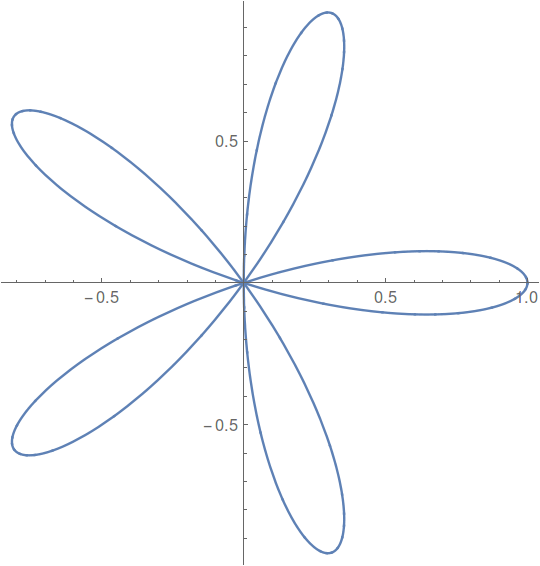
\includegraphics[scale=0.3]{Fig1.png}  
	\caption{Regi\~{a}o $ D_{xyz} = \lbrace(x, y, z)\mid x^2 + y^2 + (z-2)^2 \leq 4 $, $z \geq \sqrt{\frac{1}{3}(x^2 + y^2)} $ e $ z \leq \sqrt{x^2 + y^2} \geq 0 \rbrace $}
	\label{fig:figura1}
\end{figure}

Realizamos a seguinte mudança de coordenadas:
\begin{equation}
\left\{\begin{array}{ll}
x=\rho\sin\phi\,\cos\theta\\
y= 2\rho\sin\phi\,\sin\theta\\
z = \rho\cos\phi
\end{array}\right.
\label{eq:Q1_mudanca}
\end{equation}

\begin{equation}
|J| = \Big| \frac{\partial (x,y,z) }{\partial (\rho,\phi,\theta)} \Big| = \begin{Vmatrix}
\sin\phi\,\cos\theta &  \rho\cos\phi\,\cos\theta & -\rho\sin\phi\,\sin\theta \\
2\sin\phi\,\sin\theta & 2\rho\cos\phi\,\sin\theta & 2\rho\sin\phi\,\cos\theta \\
\cos\phi & -\rho\sin\phi & 0 \\
\end{Vmatrix} = 2\rho^2\sin\phi
\label{eq:Q1_Jac}
\end{equation}

Aplicando \eqref{eq:Q1_mudanca} \`a equaç\~{a}o da esfera:
\begin{equation}
\rho^2 = 4\rho\cos\phi \therefore \rho = 4\cos\phi
\label{eq:Q1_elipsoide}
\end{equation}

Aplicando \eqref{eq:Q1_mudanca} \`a equaç\~{a}o do cone de baixo :
\begin{equation}
\rho^2\cos^2\phi = \frac{1}{3} \rho^ 2 \sin^2\phi \Rightarrow \tan^2 \phi = 3 \therefore \phi = \frac{\pi}{3}
\label{eq:Q1_cone}
\end{equation}

Aplicando \eqref{eq:Q1_mudanca} \`a equaç\~{a}o do cone de cima :
\begin{equation}
\rho^2\cos^2\phi =  \rho^ 2 \sin^2\phi \Rightarrow \tan^2 \phi = 1 \therefore \phi = \frac{\pi}{4}
\label{eq:Q1_cone2}
\end{equation}


Assim podemos facilmente descrever $D$ em coordenadas esf\'{e}ricas. \\

Calculando a integral : \

$$ \iiint_{D_{xyz}}{z}\;dx\,dy\,dz  = \int\limits_{0}^{2\pi} \int\limits_{\frac{\pi}{4}}^{\frac{\pi}{3}}  \int\limits_{0}^{4\cos\phi} \rho \cos \phi \cdot \rho^2 \sin\phi \;d\rho\, d\phi\,d\theta $$

$$ = \int\limits_{0}^{2\pi} \int\limits_{\frac{\pi}{4}}^{\frac{\pi}{3}}  \frac{\rho^4}{4} \Big|_{0}^{4\cos\phi} \sin \phi \cos \phi \;d\phi\,d\theta = \frac{4^4}{4} \int\limits_{0}^{2\pi} \int\limits_{\frac{\pi}{4}}^{\frac{\pi}{3}}  \cos^5\phi \sin \phi \;d\phi\,d\theta  $$

Fazendo a seguinte mudaça de variável: $u = \cos\phi \Rightarrow du = -\sin\phi \, d\phi $, temos:

$$ = -4^3 \int\limits_{0}^{2\pi} \int\limits_{\frac{\sqrt{2}}{2}}^{\frac{1}{2}}  u^5 \;du\,d\theta = 4^3 \int\limits_{0}^{2\pi}  \frac{u^6}{6} \Big|_{\frac{1}{2}}^{\frac{\sqrt{2}}{2}} \;d\theta = \frac{4^3}{6} \Big( \frac{1}{8} - \frac{1}{64} \Big) \int\limits_{0}^{2\pi} \; d\theta= \frac{4^3}{6} \cdot \frac{7}{64} \cdot 2 \pi = \frac{7\pi}{3} $$

%%%%%%%%%%%%%%%%%%%%%%%%%%%%%%%%%%%%%%%%%%TURMA B%%%%%%%%%%%%%%%%%%%%%%%%%%%%%%%%%%%%%%%%%%%%%%%

\newpage
\begin{center}
\textbf{Instituto de Matemática e Estatística da USP\\
MAT2455 - Cálculo Diferencial e Integral IV para Engenharia\\}
\textbf{1a. Prova - 2o. Semestre 2015 - 07/04/2015}
\end{center}

\noindent {\bf Turma B}

%---------------------------------------QUESTAO 1-----------------------------------------

\noindent{\bf 1ª Questão:}
\begin{itemize}
	\item[a)] (1,5) Calcule a área de um laço da rosácea cuja equação em coordenadas polares é $r(\theta) = \cos 5\theta$. \\
	\item[b)] (2,0) Calcule  $\displaystyle\iint_D \frac{x+y-1}{x+y+1}\; \, dx \, dy$, sendo $D$ a região do plano limitada por:
	$$ x+y-1 = x-y+1, \; x+y-1= 2(x-y+1), \; x-y+1=1, \; x-y+1 = 2.$$
	
\end{itemize}


\noindent{\bf \\ \\Solução:}
\begin{itemize}
    \item[a)] O laço da rosácea em questão apresenta o seguinte formato:
    

\begin{figure}[h!]
	\centering
	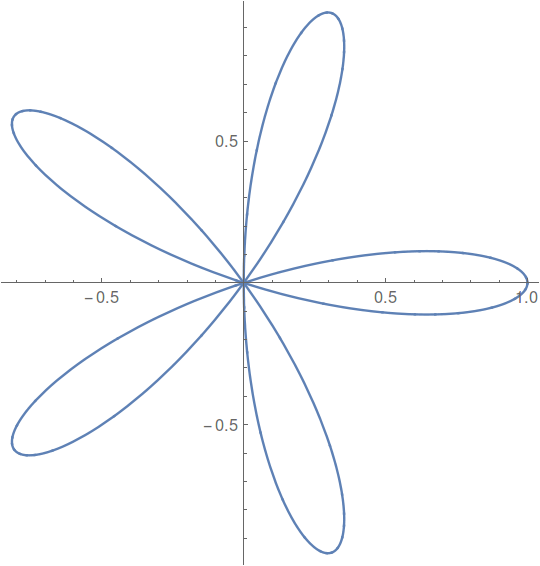
\includegraphics[scale=0.40]{Fig1.png}  
	\caption{Laço da rosácea}
	\label{fig:figura1}
\end{figure}

Como cada laço começa e termina em $r=0$ e $r \geq 0 \Rightarrow \cos 5\theta \geq 0$, deve existir um laço em $-\frac{\pi}{2} \leq 5\theta \leq \frac{\pi}{2} \Rightarrow -\frac{\pi}{10} \leq \theta \leq \frac{\pi}{10}$. Logo, a área de um laço da rosácea é dada por:

$$ \int\limits_{-\frac{\pi}{10}}^{\frac{\pi}{10}} \int\limits_0^{\cos 5\theta} \rho \; d\rho \, d\theta = \int\limits_{-\frac{\pi}{10}}^{\frac{\pi}{10}} \frac{\rho^2}{2} \Big|_0^{\cos 5\theta} \; d\theta = \frac{1}{2} \int\limits_{-\frac{\pi}{10}}^{\frac{\pi}{10}} \cos^2(5\theta) \; d\theta = \frac{1}{2} \int\limits_{-\frac{\pi}{10}}^{\frac{\pi}{10}} \frac{1 + \cos (10\theta)}{2} \; d\theta $$
$$ = \frac{1}{4} \Big( \theta + \frac{\sin (10\theta)}{10} \Big)_{-\frac{\pi}{10}}^{\frac{\pi}{10}} = \frac{1}{4} \cdot \frac{\pi}{5} = \frac{\pi}{20} $$

\item[b)] O domínio de integração é exibido abaixo

\begin{figure}[H]
	\centering
	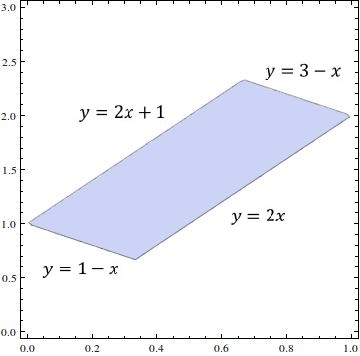
\includegraphics[scale=0.4]{Q1bA.jpg}  
	\caption{Domínio de integração}
	\label{fig:figura2}
\end{figure}    
Faz-se a seguinte mudança de coordenadas:
$$\begin{cases}
u = x+y-1\\
v = x-y+1
\end{cases}
\Rightarrow
\begin{cases}
x = \frac{u+v}{2}\\
y = \frac{u-v}{2}+1
\end{cases}
$$

O jacobiano da transformação é dado por:
$$
\frac{\partial(x,y)}{\partial(u,v)}=
\begin{vmatrix}
\frac{1}{2} & \frac{1}{2} \\
\frac{1}{2} & -\frac{1}{2}\\
\end{vmatrix}
=-\frac{1}{2} \Rightarrow |J|=\frac{1}{2}\\
$$  

O novo domínio de integração é exibido abaixo

\begin{figure}[h!]
	\centering
	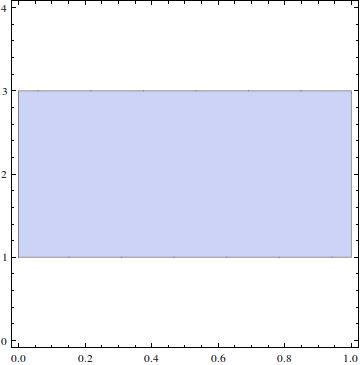
\includegraphics[scale=0.4]{Q1b2A.jpg}  
	\caption{Domínio de integração após mudança}
	\label{fig:figura3}
\end{figure}
E passa a ser dado por:

$$D(u,v)=\{(u,v)\in \re^2|v \leq u \leq 2v\,\,\mbox{,}\,\,1 \leq v \leq 2 \}$$

A integral a ser calculada passa a ser:

$$ \int\limits_1^2 \int\limits_v^{2v} \frac{u}{v^4} \cdot \frac{1}{2} \; du \, dv = \frac{1}{2} \int\limits_1^2  \frac{u^2}{2} \Big|_v^{2v} \frac{1}{v^4}  \; dv = \frac{1}{4} \int\limits_1^2  \frac{4v^2 - v^2}{v^4}  \; dv = \frac{3}{4} \int\limits_1^2  \frac{1}{v^2}  \; dv = \frac{3}{4} \cdot \frac{v^{-1}}{-1} \Big|_1^2 = -\frac{3}{4} \Big( \frac{1}{2} -1 \Big) = \frac{3}{8} $$

\end{itemize}

%---------------------------------------QUESTAO 2-----------------------------------------
\newpage

\noindent{\bf 2ª Questão:}

\begin{itemize}
\item[a)] (2,0) Calcule a massa da curva cujo traço é a parte da elipse $\displaystyle\frac{x^2}{3} + \displaystyle\frac{y^2}{4} = 1 $ no primeiro quadrante com densidade $\delta(x,y) = xy$. \\
\item[b)] (1,5) Inverta a ordem de integração e calcule a integral iterada: $\displaystyle\int_0^2 \int_{y^2}^4 y \frac{\ln (1+x^2)}{1+x^2} \; dx \, dy$.
\end{itemize}

\noindent{\bf Solução:} \\

\begin{itemize}
\item[a)]
Devemos calcular a integral
$$  \int_{\gamma}{\delta(x,y,z)}\;ds $$

\begin{figure}[h!]
	\centering
	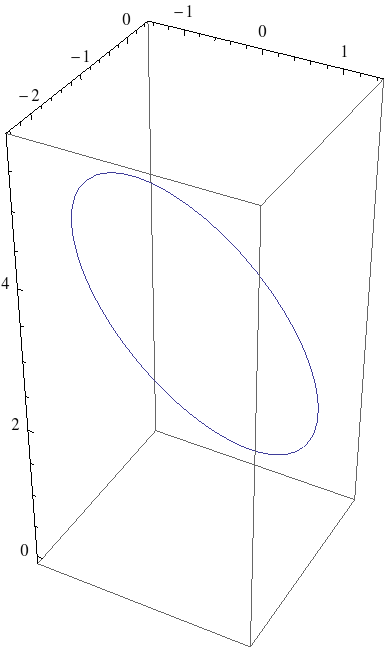
\includegraphics[scale=0.2]{Fig3.png}  
	\caption{Curva $\gamma(t)$}
	\label{fig:figura3}
\end{figure}

Parametrizando a curva em questão:

$$
\frac{x^2}{3} + \frac{y^2}{4} = 1
\Rightarrow
\begin{cases}
x(t) = \sqrt{3}\cos t \\
y(t) = 2\sin t\\
\end{cases}
$$

$$ \therefore \gamma(t) = (\sqrt{3}\cos t, 2\sin t), t \in \Big[0,\frac{\pi}{2}\Big] $$
$$ \gamma'(t) = (-\sqrt{3}\sin t, 2\cos t) $$
$$ ||\gamma'(t)|| = \sqrt{3\sin^2 t + 4\cos^2 t} = \sqrt{1 + \cos^2 t} $$

Utilizando a definição de integral de linha de uma função escalar:

$$  \int_{\gamma}{\delta(x,y)}\;ds = \int_{t_i}^{t_f} {\delta(\gamma(t)) ||\gamma'(t) ||}\;dt = \int_{0}^{\frac{\pi}{2}} 2 \sqrt{3} \, \sin t \cos t \sqrt{1 + \cos^2 t} \;dt $$

Utilizando a seguinte mudança de váriavel: $u = 1 + \cos^2 t \Rightarrow du = -2\cos t \sin t \; dt $, temos:

$$ = -\sqrt{3} \int_1^0 \sqrt{u} \; du =  \sqrt{3} \int_0^1 \sqrt{u} \; du = \sqrt{3} \, \frac{2u^{\frac{3}{2}}}{3} \Big|_0^1 = \frac{2\sqrt{3}}{3} $$

\item[b)] $$ \int_0^2 \int_{y^2}^4 y \frac{\ln (1+x^2)}{1+x^2} \; dx \, dy = \int_0^4 \int_0^{\sqrt{x}} y \frac{\ln (1+x^2)}{1+x^2} \; dy \, dx  $$
$$ = \int_0^4  \frac{y^2}{2} \Big|_0^{\sqrt{x}} \, \frac{\ln (1+x^2)}{1+x^2} \; dx = \frac{1}{2} \int_0^4 x \frac{\ln (1+x^2)}{1+x^2} \; dx $$
Utilizando a seguinte mudança de váriavel: $u = 1 + 1+x^2 \Rightarrow du = 2 x \; dx $, temos:
$$ =  \frac{1}{4} \int_1^{17} \frac{\ln (u)}{u} \; du $$
Integrando por partes, temos:
$$ \int \frac{\ln (u)}{u} \; du = \ln^2 u - \int \frac{\ln (u)}{u} \; du \therefore \int \frac{\ln (u)}{u} \; du = \frac{\ln^2 u}{2} + C $$
$$ \therefore \frac{1}{4} \int_1^{17} \frac{\ln (u)}{u} \; du = \frac{1}{8} \ln^2 u \Big|_1^{17} = \frac{\ln^2(17)}{8} $$

\end{itemize}

%---------------------------------------QUESTAO 3-----------------------------------------
\newpage

\noindent{\bf 3ª Questão:} (3,0) \\

Calcule a massa do sólido que é parte da bola $ x^2 + y^2 + (z-2)^2 \leq 4 $, acima do cone $ z = \displaystyle\sqrt{\frac{1}{3}(x^2 + y^2)}$ e abaixo do cone $z = \sqrt{x^2 + y^2}$, com densidade $\delta(x,y,z) = z$. \\

\noindent{\bf Solução:}
\\

Devemos calcular a integral
\begin{equation}
 \iiint_{D_{xyz}} z \;dx\,dy\,dz \
\label{eq:integral}
\end{equation}

\begin{figure}[h!]
	\centering
	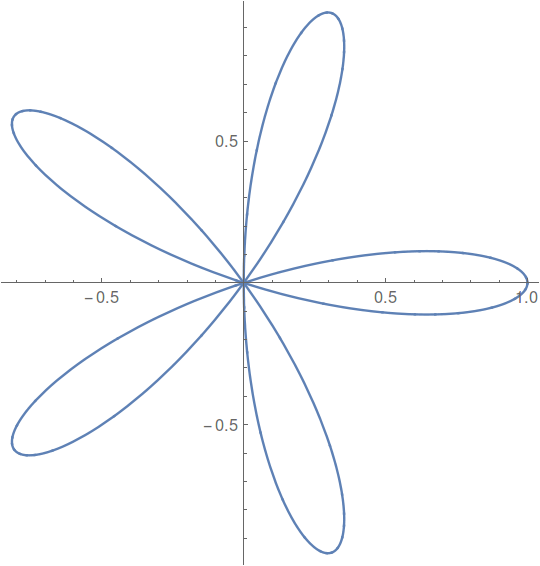
\includegraphics[scale=0.3]{Fig1.png}  
	\caption{Regi\~{a}o $ D_{xyz} = \lbrace(x, y, z)\mid x^2 + y^2 + (z-2)^2 \leq 4 $, $z \geq \sqrt{\frac{1}{3}(x^2 + y^2)} $ e $ z \leq \sqrt{x^2 + y^2} \geq 0 \rbrace $}
	\label{fig:figura1}
\end{figure}

Realizamos a seguinte mudança de coordenadas:
\begin{equation}
\left\{\begin{array}{ll}
x=\rho\sin\phi\,\cos\theta\\
y= 2\rho\sin\phi\,\sin\theta\\
z = \rho\cos\phi
\end{array}\right.
\label{eq:Q1_mudanca}
\end{equation}

\begin{equation}
|J| = \Big| \frac{\partial (x,y,z) }{\partial (\rho,\phi,\theta)} \Big| = \begin{Vmatrix}
\sin\phi\,\cos\theta &  \rho\cos\phi\,\cos\theta & -\rho\sin\phi\,\sin\theta \\
2\sin\phi\,\sin\theta & 2\rho\cos\phi\,\sin\theta & 2\rho\sin\phi\,\cos\theta \\
\cos\phi & -\rho\sin\phi & 0 \\
\end{Vmatrix} = 2\rho^2\sin\phi
\label{eq:Q1_Jac}
\end{equation}

Aplicando \eqref{eq:Q1_mudanca} \`a equaç\~{a}o da esfera:
\begin{equation}
\rho^2 = 4\rho\cos\phi \therefore \rho = 4\cos\phi
\label{eq:Q1_elipsoide}
\end{equation}

Aplicando \eqref{eq:Q1_mudanca} \`a equaç\~{a}o do cone de baixo :
\begin{equation}
\rho^2\cos^2\phi = \frac{1}{3} \rho^ 2 \sin^2\phi \Rightarrow \tan^2 \phi = 3 \therefore \phi = \frac{\pi}{3}
\label{eq:Q1_cone}
\end{equation}

Aplicando \eqref{eq:Q1_mudanca} \`a equaç\~{a}o do cone de cima :
\begin{equation}
\rho^2\cos^2\phi =  \rho^ 2 \sin^2\phi \Rightarrow \tan^2 \phi = 1 \therefore \phi = \frac{\pi}{4}
\label{eq:Q1_cone2}
\end{equation}


Assim podemos facilmente descrever $D$ em coordenadas esf\'{e}ricas. \\

Calculando a integral : \

$$ \iiint_{D_{xyz}}{z}\;dx\,dy\,dz  = \int\limits_{0}^{2\pi} \int\limits_{\frac{\pi}{4}}^{\frac{\pi}{3}}  \int\limits_{0}^{4\cos\phi} \rho \cos \phi \cdot \rho^2 \sin\phi \;d\rho\, d\phi\,d\theta $$

$$ = \int\limits_{0}^{2\pi} \int\limits_{\frac{\pi}{4}}^{\frac{\pi}{3}}  \frac{\rho^4}{4} \Big|_{0}^{4\cos\phi} \sin \phi \cos \phi \;d\phi\,d\theta = \frac{4^4}{4} \int\limits_{0}^{2\pi} \int\limits_{\frac{\pi}{4}}^{\frac{\pi}{3}}  \cos^5\phi \sin \phi \;d\phi\,d\theta  $$

Fazendo a seguinte mudaça de variável: $u = \cos\phi \Rightarrow du = -\sin\phi \, d\phi $, temos:

$$ = -4^3 \int\limits_{0}^{2\pi} \int\limits_{\frac{\sqrt{2}}{2}}^{\frac{1}{2}}  u^5 \;du\,d\theta = 4^3 \int\limits_{0}^{2\pi}  \frac{u^6}{6} \Big|_{\frac{1}{2}}^{\frac{\sqrt{2}}{2}} \;d\theta = \frac{4^3}{6} \Big( \frac{1}{8} - \frac{1}{64} \Big) \int\limits_{0}^{2\pi} \; d\theta= \frac{4^3}{6} \cdot \frac{7}{64} \cdot 2 \pi = \frac{7\pi}{3} $$

\end{document} 
